\documentclass[10pt]{article}
\usepackage[utf8]{inputenc}
\usepackage[portuguese]{babel}

\title{IF684 - Sistemas Inteligentes}
\author{José Antônio Alves Maciel}
\date{May 2019}

\usepackage{natbib}
\usepackage{graphicx}

\begin{document}

\maketitle

\section{Introdução}
Sistemas Inteligentes é uma cadeira obrigatória com 75 horas de carga horária e aborda áreas como Inteligência Artificial, Redes Neurais e Aprendizagem de Máquinas. O objetivo da disciplina encontra-se no estudo de técnicas computacionais que apresentem características de aprendizagem automática, através do fornecimento de uma visão geral da área de aprendizagem de máquina e do estudo dos métodos e técnicas de aprendizagem simbólica, conexionista e evolucionista.
\cite{intro}


\begin{figure}[h!]
\centering
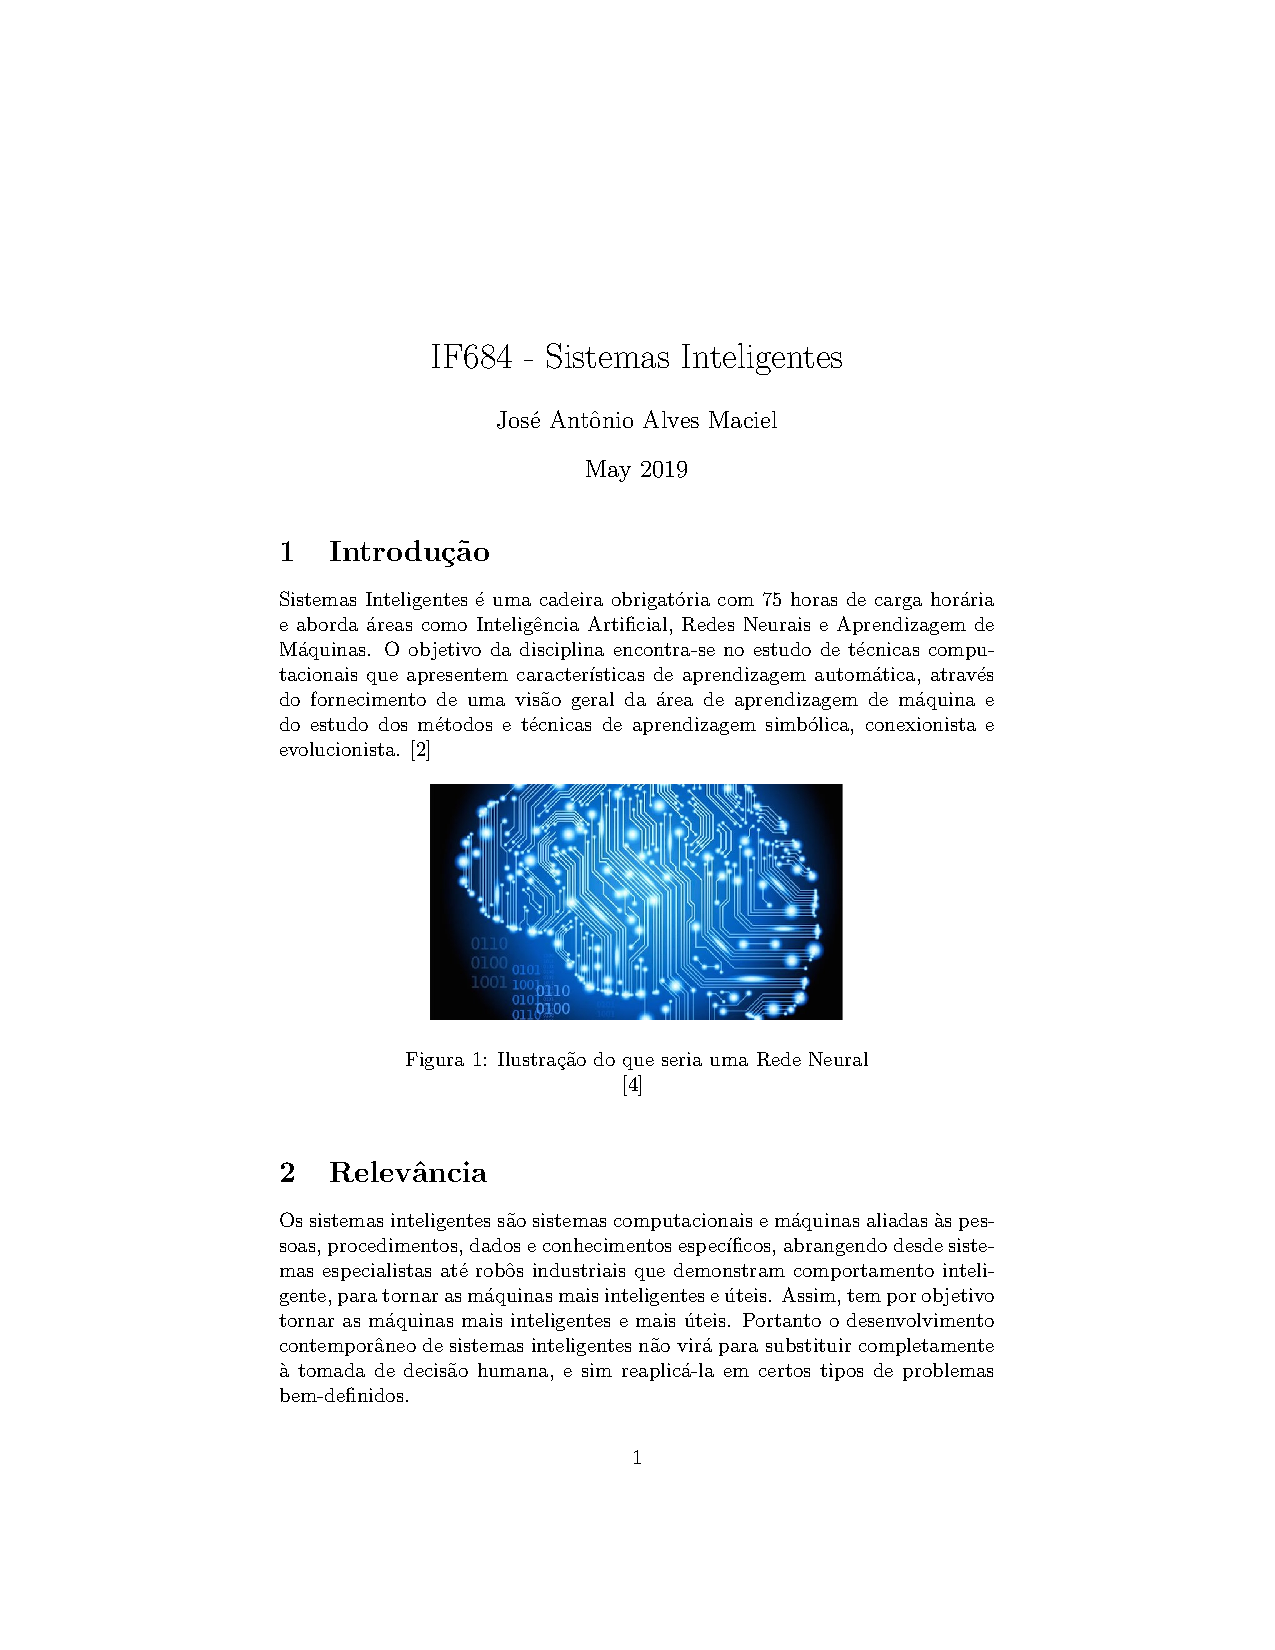
\includegraphics[scale=0.3]{jaam.jpg}
\caption{Ilustração do que seria uma Rede Neural}\cite{imagem}
\label{fig:jaam}
\end{figure}

\section{Relevância}
Os sistemas inteligentes são sistemas computacionais e máquinas aliadas às pessoas, procedimentos, dados e conhecimentos específicos, abrangendo desde sistemas especialistas até robôs industriais que demonstram comportamento inteligente, para tornar as máquinas mais inteligentes e úteis. Assim, tem por objetivo tornar as máquinas mais inteligentes e mais úteis. Portanto o desenvolvimento contemporâneo de sistemas inteligentes não virá para substituir completamente à tomada de decisão humana, e sim reaplicá-la em certos tipos de problemas bem-definidos.


\section{Disciplinas Relacionadas}
\begin{table}[h]
\begin{tabular}{lllll}
\cline{1-2}
\multicolumn{1}{|c|}{IF699 - Aprendizagem de Máquina} & \multicolumn{1}{l|}{\begin{tabular}[c]{@{}l@{}}Nessa disciplina, são aprendidos méto-\\dos e algoritmos que obtém conheci-\\ mentos a partir da análise de bases de \\dados, uma habilidade essencial para\\ o desenvolvimento de uma IA.\citep{BibliografiadeSistemasInteligentes1}\end{tabular}} &  &  &  \\ \cline{1-2}
\multicolumn{1}{|l|}{IF702 - Redes Neurais} & \multicolumn{1}{l|}{\begin{tabular}[c]{@{}l@{}}Nessa disciplina, é ensinado o uso de\\ algoritmos em sistemas\\  para que possam reconhecer padrões \\ e dados correlacionados afim de \\agrupá-los e classificá-los, e, com \\o tempo, aprender e melhorar continua-\\mente.Dessa forma se relacionando\\ profundamente com sistemas\\ inteligentes.\cite{BibliografiadeSistemasInteligentes2}\end{tabular}} &  &  &  \\ \cline{1-2}
 &  &  &  &  \\
 &  &  &  & 
\end{tabular}
\end{table}

\bibliographystyle{plain}
\bibliography{jaam}
\end{document}